\FChapter{Chapter Thirty-Three}{33}

\Lettrine{W}{hen} \textsc{\Mr{} \St{} John went,} it was beginning to snow; the whirling storm
continued all night. The next day a keen wind brought fresh and
blinding falls; by twilight the valley was drifted up and almost
impassable. I had closed my shutter, laid a mat to the door to prevent
the snow from blowing in under it, trimmed my fire, and after sitting
nearly an hour on the hearth listening to the muffled fury of the
tempest, I lit a candle, took down \enquote{Marmion,} and beginning---

\settoversewidth{\versewidth}{The flanking walls that round them sweep,}
\begin{verse}[\versewidth]
\enquote{Day set on Norham's castled steep,\\*
And Tweed's fair river broad and deep,\\*
\hspace*{0.333em}\hspace*{0.333em} And Cheviot's mountains lone;\\*
The massive towers, the donjon keep,\\*
The flanking walls that round them sweep,\\*
\hspace*{0.333em}\hspace*{0.333em} In yellow lustre shone}---
\end{verse}

I soon forgot storm in music.

I heard a noise: the wind, I thought, shook the door. No; it was St.
John Rivers, who, lifting the latch, came in out of the frozen
hurricane---the howling darkness---and stood before me: the cloak that
covered his tall figure all white as a glacier. I was almost in
consternation, so little had I expected any guest from the blocked-up
vale that night.

\enquote{Any ill news?} I demanded. \enquote{Has anything happened?}

\enquote{No. How very easily alarmed you are!} he answered, removing
his cloak and hanging it up against the door, towards which he again
coolly pushed the mat which his entrance had deranged. He stamped the
snow from his boots.

\enquote{I shall sully the purity of your floor,} said he, \enquote{but
you must excuse me for once.} Then he approached the fire. \enquote{I
have had hard work to get here, I assure you,} he observed, as he warmed
his hands over the flame. \enquote{One drift took me up to the waist;
happily the snow is quite soft yet.}

\enquote{But why are you come?} I could not forbear saying.

\enquote{Rather an inhospitable question to put to a visitor; but since
you ask it, I answer simply to have a little talk with you; I got tired
of my mute books and empty rooms. Besides, since yesterday I have
experienced the excitement of a person to whom a tale has been
half-told, and who is impatient to hear the sequel.}

He sat down. I recalled his singular conduct of yesterday, and really I
began to fear his wits were touched. If he were insane, however, his
was a very cool and collected insanity: I had never seen that
handsome-featured face of his look more like chiselled marble than it
did just now, as he put aside his snow-wet hair from his forehead and
let the firelight shine free on his pale brow and cheek as pale, where
it grieved me to discover the hollow trace of care or sorrow now so
plainly graved. I waited, expecting he would say something I could at
least comprehend; but his hand was now at his chin, his finger on his
lip: he was thinking. It struck me that his hand looked wasted like his
face. A perhaps uncalled-for gush of pity came over my heart: I was
moved to say---

\enquote{I wish Diana or Mary would come and live with you: it is too
bad that you should be quite alone; and you are recklessly rash about
your own health.}

\enquote{Not at all,} said he: \enquote{I care for myself when
necessary. I am well now. What do you see amiss in me?}

This was said with a careless, abstracted indifference, which showed
that my solicitude was, at least in his opinion, wholly superfluous. I
was silenced.

He still slowly moved his finger over his upper lip, and still his eye
dwelt dreamily on the glowing grate; thinking it urgent to say
something, I asked him presently if he felt any cold draught from the
door, which was behind him.

\enquote{No, no!} he responded shortly and somewhat testily.

\enquote{Well,} I reflected, \enquote{if you won't talk, you may be
still; I'll let you alone now, and return to my book.}

So I snuffed the candle and resumed the perusal of \enquote{Marmion.} 
He soon stirred; my eye was instantly drawn to his movements; he only
took out a morocco pocket-book, thence produced a letter, which he read
in silence, folded it, put it back, relapsed into meditation. It was
vain to try to read with such an inscrutable fixture before me; nor
could I, in impatience, consent to be dumb; he might rebuff me if he
liked, but talk I would.

\enquote{Have you heard from Diana and Mary lately?}

\enquote{Not since the letter I showed you a week ago.}

\enquote{There has not been any change made about your own
arrangements? You will not be summoned to leave England sooner than you
expected?}

\enquote{I fear not, indeed: such chance is too good to befall me.} 
Baffled so far, I changed my ground. I bethought myself to talk about
the school and my scholars.

\enquote{Mary Garrett's mother is better, and Mary came back to the
school this morning, and I shall have four new girls next week from the
Foundry Close---they would have come to-day but for the snow.}

\enquote{Indeed!}

\enquote{\Mr{} Oliver pays for two.}

\enquote{Does he?}

\enquote{He means to give the whole school a treat at Christmas.}

\enquote{I know.}

\enquote{Was it your suggestion?}

\enquote{No.}

\enquote{Whose, then?}

\enquote{His daughter's, I think.}

\enquote{It is like her: she is so good-natured.}

\enquote{Yes.}

Again came the blank of a pause: the clock struck eight strokes. It
aroused him; he uncrossed his legs, sat erect, turned to me.

\enquote{Leave your book a moment, and come a little nearer the fire,}
he said.

Wondering, and of my wonder finding no end, I complied.

\enquote{Half-an-hour ago,} he pursued, \enquote{I spoke of my impatience to
hear the sequel of a tale: on reflection, I find the matter will be
better managed by my assuming the narrator's part, and converting you
into a listener. Before commencing, it is but fair to warn you that the
story will sound somewhat hackneyed in your ears; but stale details
often regain a degree of freshness when they pass through new lips. For
the rest, whether trite or novel, it is short.

%rem enq
Twenty years ago, a poor curate---never mind his name at this
moment---fell in love with a rich man's daughter; she fell in love with
him, and married him, against the advice of all her friends, who
consequently disowned her immediately after the wedding. Before two
years passed, the rash pair were both dead, and laid quietly side by
side under one slab. (I have seen their grave; it formed part of the
pavement of a huge churchyard surrounding the grim, soot-black old
cathedral of an overgrown manufacturing town in ---shire.) They left a
daughter, which, at its very birth, Charity received in her lap---cold
as that of the snow-drift I almost stuck fast in to-night. Charity
carried the friendless thing to the house of its rich maternal
relations; it was reared by an aunt-in-law, called (I come to names now)
\Mrs{} Reed of Gateshead. You start---did you hear a noise? I daresay it
is only a rat scrambling along the rafters of the adjoining schoolroom:
it was a barn before I had it repaired and altered, and barns are
generally haunted by rats.---To proceed. \Mrs{} Reed kept the orphan ten
years: whether it was happy or not with her, I cannot say, never having
been told; but at the end of that time she transferred it to a place you
know---being no other than Lowood School, where you so long resided
yourself. It seems her career there was very honourable: from a pupil,
she became a teacher, like yourself---really it strikes me there are
parallel points in her history and yours---she left it to be a
governess: there, again, your fates were analogous; she undertook the
education of the ward of a certain \Mr{} Rochester.}

\enquote{\Mr{} Rivers!} I interrupted.

\enquote{I can guess your feelings,} he said, \enquote{but restrain them
for a while: I have nearly finished; hear me to the end. Of \Mr{}
 Rochester's character I know nothing, but the one fact that he professed
to offer honourable marriage to this young girl, and that at the very
altar she discovered he had a wife yet alive, though a lunatic. What
his subsequent conduct and proposals were is a matter of pure
conjecture; but when an event transpired which rendered inquiry after
the governess necessary, it was discovered she was gone---no one could
tell when, where, or how. She had left Thornfield Hall in the night;
every research after her course had been vain: the country had been
scoured far and wide; no vestige of information could be gathered
respecting her. Yet that she should be found is become a matter of
serious urgency: advertisements have been put in all the papers; I
myself have received a letter from one \Mr{} Briggs, a solicitor,
communicating the details I have just imparted. Is it not an odd tale?}

\enquote{Just tell me this,} said I, \enquote{and since you know so
much, you surely can tell it me---what of \Mr{} Rochester? How and where
is he? What is he doing? Is he well?}

\enquote{I am ignorant of all concerning \Mr{} Rochester: the letter never
mentions him but to narrate the fraudulent and illegal attempt I have
adverted to. You should rather ask the name of the governess---the
nature of the event which requires her appearance.}

\enquote{Did no one go to Thornfield Hall, then? Did no one see \Mr{}
 Rochester?}

\enquote{I suppose not.}

\enquote{But they wrote to him?}

\enquote{Of course.}

\enquote{And what did he say? Who has his letters?}

\enquote{\Mr{} Briggs intimates that the answer to his application was not
from \Mr{} Rochester, but from a lady: it is signed \enquote{Alice
Fairfax.}}

I felt cold and dismayed: my worst fears then were probably true: he had
in all probability left England and rushed in reckless desperation to
some former haunt on the Continent. And what opiate for his severe
sufferings---what object for his strong passions---had he sought there? 
I dared not answer the question. Oh, my poor master---once almost my
husband---whom I had often called \enquote{my dear Edward!}

\enquote{He must have been a bad man,} observed \Mr{} Rivers.

\enquote{You don't know him---don't pronounce an opinion upon him,} I
said, with warmth.

\enquote{Very well,} he answered quietly: \enquote{and indeed my head is
otherwise occupied than with him: I have my tale to finish. Since you
won't ask the governess's name, I must tell it of my own accord. Stay! 
I have it here---it is always more satisfactory to see important points
written down, fairly committed to black and white.}

And the pocket-book was again deliberately produced, opened, sought
through; from one of its compartments was extracted a shabby slip of
paper, hastily torn off: I recognised in its texture and its stains of
ultra-marine, and lake, and vermillion, the ravished margin of the
portrait-cover. He got up, held it close to my eyes: and I read, traced
in Indian ink, in my own handwriting, the words \enquote{{Jane Eyre}}---the
work doubtless of some moment of abstraction.

\enquote{Briggs wrote to me of a Jane Eyre:} he said, \enquote{the
advertisements demanded a Jane Eyre: I knew a Jane Elliott.---I confess
I had my suspicions, but it was only yesterday afternoon they were at
once resolved into certainty. You own the name and renounce the
\emph{alias}?}

\enquote{Yes---yes; but where is \Mr{} Briggs? He perhaps knows more of
\Mr{} Rochester than you do.}

\enquote{Briggs is in London. I should doubt his knowing anything at
all about \Mr{} Rochester; it is not in \Mr{} Rochester he is interested. 
Meantime, you forget essential points in pursuing trifles: you do not
inquire why \Mr{} Briggs sought after you---what he wanted with you.}

\enquote{Well, what did he want?}

\enquote{Merely to tell you that your uncle, \Mr{} Eyre of Madeira, is
dead; that he has left you all his property, and that you are now
rich---merely that---nothing more.}

\enquote{I!---rich?}

\enquote{Yes, you, rich---quite an heiress.}

Silence succeeded.

\enquote{You must prove your identity of course,} resumed \St{} John
presently: \enquote{a step which will offer no difficulties; you can
then enter on immediate possession. Your fortune is vested in the
English funds; Briggs has the will and the necessary documents.}

Here was a new card turned up! It is a fine thing, reader, to be lifted
in a moment from indigence to wealth---a very fine thing; but not a
matter one can comprehend, or consequently enjoy, all at once. And then
there are other chances in life far more thrilling and rapture-giving:
\emph{this} is solid, an affair of the actual world, nothing ideal about
it: all its associations are solid and sober, and its manifestations are
the same. One does not jump, and spring, and shout hurrah! at hearing
one has got a fortune; one begins to consider responsibilities, and to
ponder business; on a base of steady satisfaction rise certain grave
cares, and we contain ourselves, and brood over our bliss with a solemn
brow.

Besides, the words Legacy, Bequest, go side by side with the words,
Death, Funeral. My uncle I had heard was dead---my only relative; ever
since being made aware of his existence, I had cherished the hope of one
day seeing him: now, I never should. And then this money came only to
me: not to me and a rejoicing family, but to my isolated self. It was a
grand boon doubtless; and independence would be glorious---yes, I felt
that---that thought swelled my heart.

\enquote{You unbend your forehead at last,} said \Mr{} Rivers. \enquote{I
thought Medusa had looked at you, and that you were turning to stone. 
Perhaps now you will ask how much you are worth?}

\enquote{How much am I worth?}

\enquote{Oh, a trifle! Nothing of course to speak of---twenty thousand
pounds, I think they say---but what is that?}

\enquote{Twenty thousand pounds?}

Here was a new stunner---I had been calculating on four or five
thousand. This news actually took my breath for a moment: \Mr{} \St{} John,
whom I had never heard laugh before, laughed now.

\enquote{Well,} said he, \enquote{if you had committed a murder, and I
had told you your crime was discovered, you could scarcely look more
aghast.}

\enquote{It is a large sum---don't you think there is a mistake?}

\enquote{No mistake at all.}

\enquote{Perhaps you have read the figures wrong---it may be two
thousand!}

\enquote{It is written in letters, not figures,---twenty thousand.}

I again felt rather like an individual of but average gastronomical
powers sitting down to feast alone at a table spread with provisions for
a hundred. \Mr{} Rivers rose now and put his cloak on.

\enquote{If it were not such a very wild night,} he said, \enquote{I
would send Hannah down to keep you company: you look too desperately
miserable to be left alone. But Hannah, poor woman! could not stride
the drifts so well as I: her legs are not quite so long: so I must e'en
leave you to your sorrows. Good-night.}

He was lifting the latch: a sudden thought occurred to me. 
\enquote{Stop one minute!} I cried.

\enquote{Well?}

\enquote{It puzzles me to know why \Mr{} Briggs wrote to you about me; or
how he knew you, or could fancy that you, living in such an
out-of-the-way place, had the power to aid in my discovery.}

\enquote{Oh! I am a clergyman,} he said; \enquote{and the clergy are
often appealed to about odd matters.} Again the latch rattled.

\enquote{No; that does not satisfy me!} I exclaimed: and indeed there
was something in the hasty and unexplanatory reply which, instead of
allaying, piqued my curiosity more than ever.

\enquote{It is a very strange piece of business,} I added; \enquote{I
must know more about it.}

\enquote{Another time.}

\enquote{No; to-night!---to-night!} and as he turned from the door, I
placed myself between it and him. He looked rather embarrassed.

\enquote{You certainly shall not go till you have told me all,} I said.

\enquote{I would rather not just now.}

\enquote{You shall!---you must!}

\enquote{I would rather Diana or Mary informed you.}

Of course these objections wrought my eagerness to a climax: gratified
it must be, and that without delay; and I told him so.

\enquote{But I apprised you that I was a hard man,} said he,
\enquote{difficult to persuade.}

\enquote{And I am a hard woman,---impossible to put off.}

\begin{figure}
	\begin{sidecaption}{\enquote{And I am a hard woman,\linebreak---impossible to put off.}}[p369b]
		\centering
		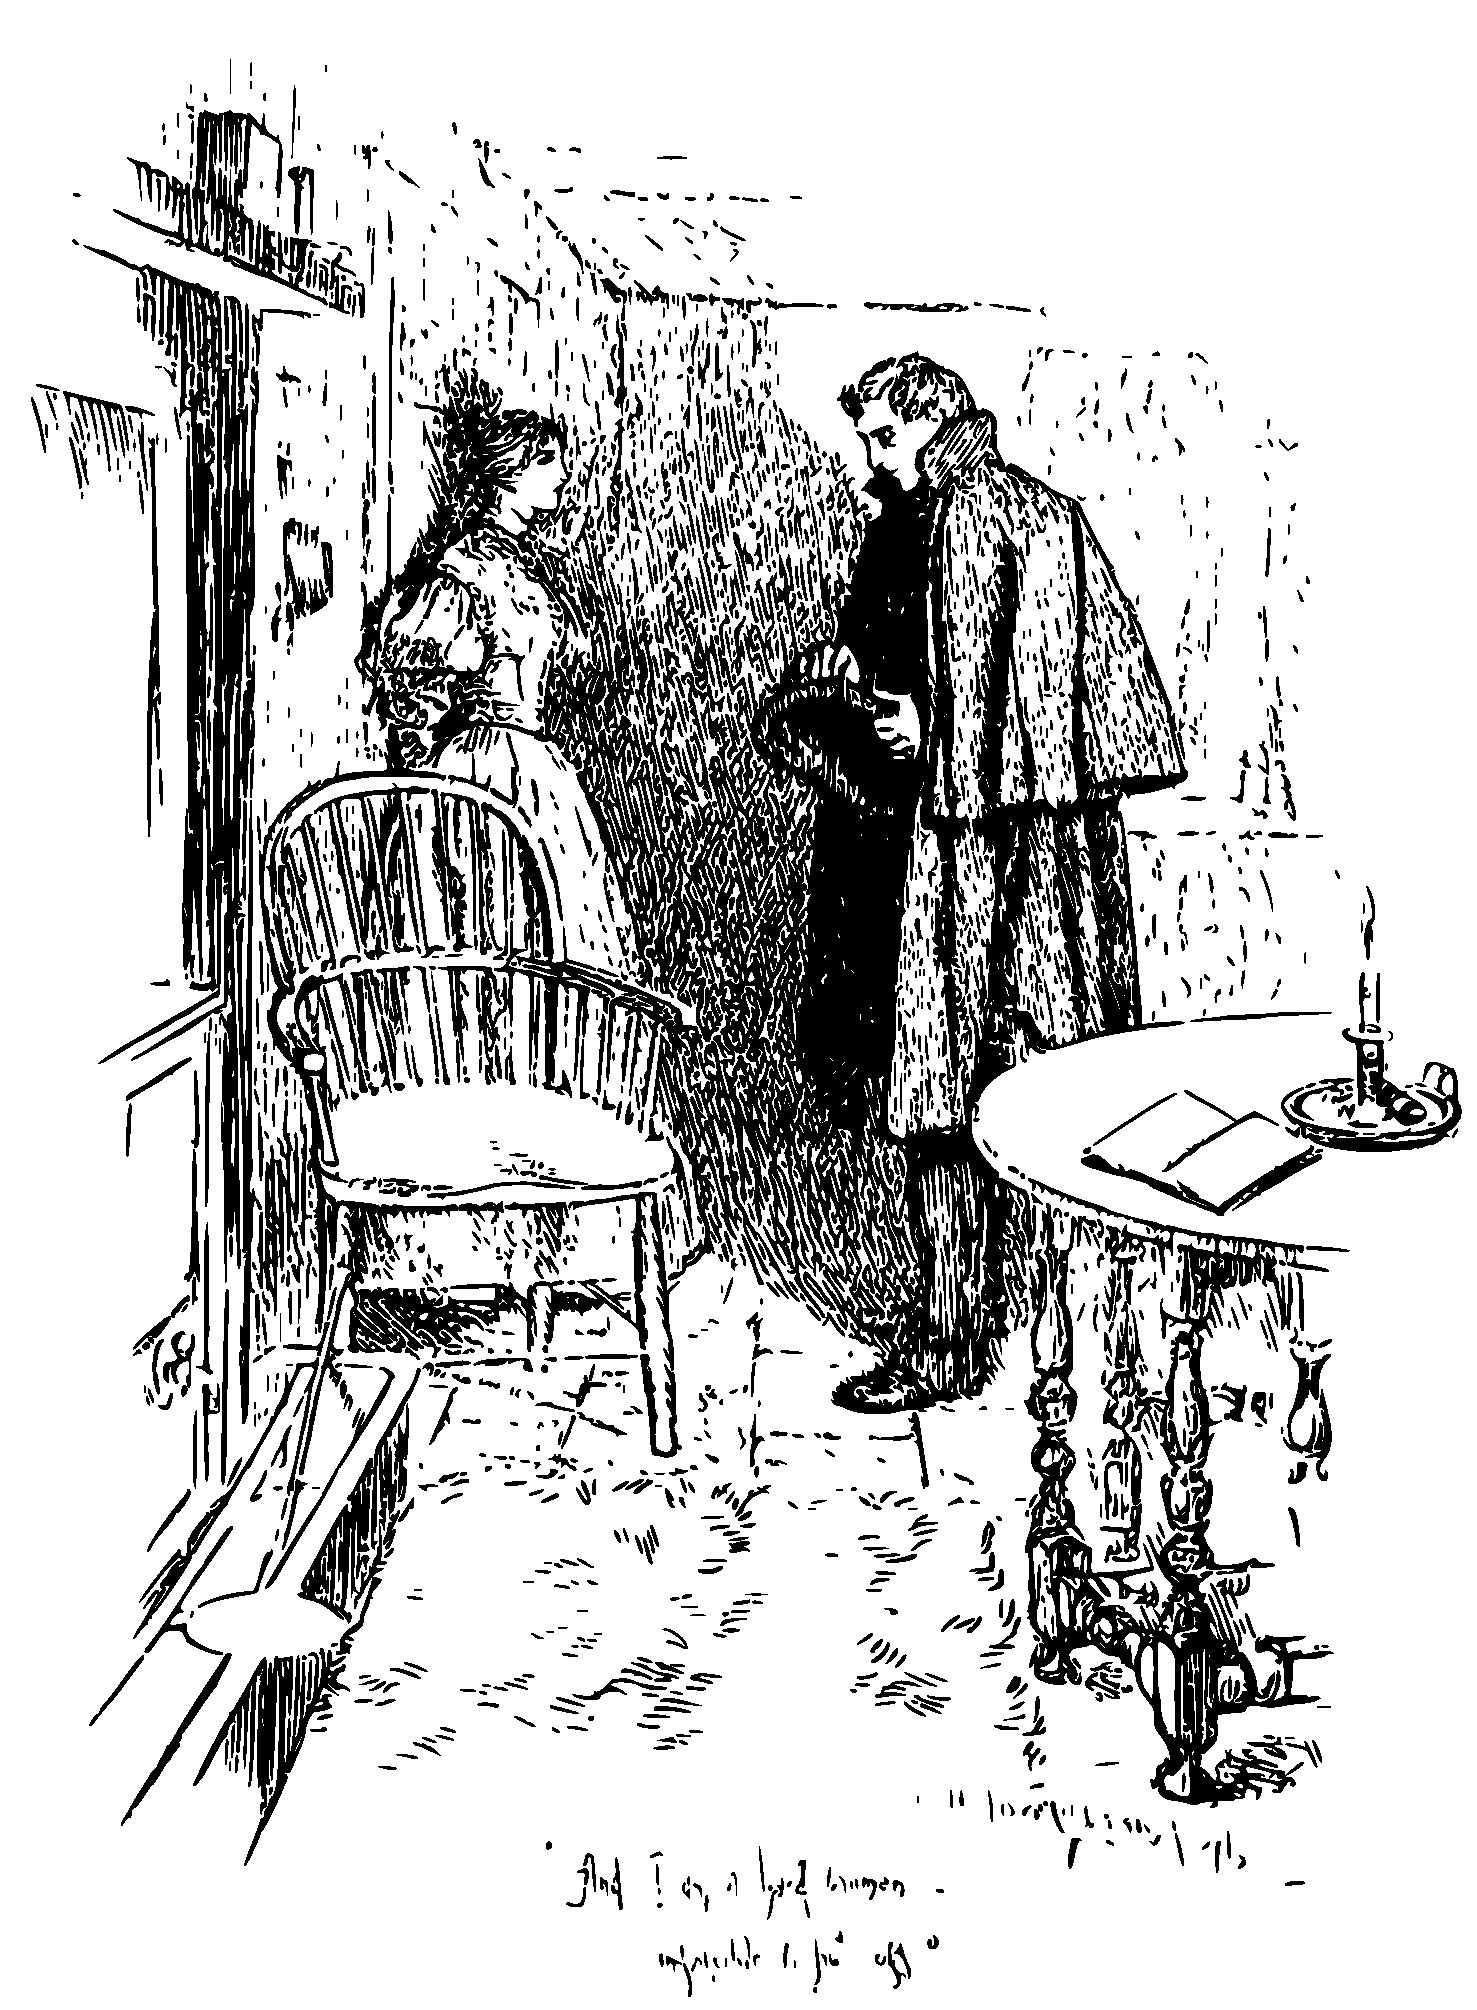
\includegraphics[width=\linewidth]{images/p369b.pdf}
	\end{sidecaption}
\end{figure}

\enquote{And then,} he pursued, \enquote{I am cold: no fervour infects
me.}

\enquote{Whereas I am hot, and fire dissolves ice. The blaze there has
thawed all the snow from your cloak; by the same token, it has streamed
on to my floor, and made it like a trampled street. As you hope ever to
be forgiven, \Mr{} Rivers, the high crime and misdemeanour of spoiling a
sanded kitchen, tell me what I wish to know.}

\enquote{Well, then,} he said, \enquote{I yield; if not to your
earnestness, to your perseverance: as stone is worn by continual
dropping. Besides, you must know some day,---as well now as later. 
Your name is Jane Eyre?}

\enquote{Of course: that was all settled before.}

\enquote{You are not, perhaps, aware that I am your namesake?---that I
was christened \St{} John Eyre Rivers?}

\enquote{No, indeed! I remember now seeing the letter E. comprised in
your initials written in books you have at different times lent me; but
I never asked for what name it stood. But what then? Surely---}

I stopped: I could not trust myself to entertain, much less to express,
the thought that rushed upon me---that embodied itself,---that, in a
second, stood out a strong, solid probability. Circumstances knit
themselves, fitted themselves, shot into order: the chain that had been
lying hitherto a formless lump of links was drawn out straight,---every
ring was perfect, the connection complete. I knew, by instinct, how the
matter stood, before \St{} John had said another word; but I cannot expect
the reader to have the same intuitive perception, so I must repeat his
explanation.

\enquote{My mother's name was Eyre; she had two brothers; one a
clergyman, who married Miss Jane Reed, of Gateshead; the other, John
Eyre, Esq., merchant, late of Funchal, Madeira. \Mr{} Briggs, being \Mr{}
Eyre's solicitor, wrote to us last August to inform us of our uncle's
death, and to say that he had left his property to his brother the
clergyman's orphan daughter, overlooking us, in consequence of a
quarrel, never forgiven, between him and my father. He wrote again a
few weeks since, to intimate that the heiress was lost, and asking if we
knew anything of her. A name casually written on a slip of paper has
enabled me to find her out. You know the rest.} Again he was going,
but I set my back against the door.

\enquote{Do let me speak,} I said; \enquote{let me have one moment to
draw breath and reflect.} I paused---he stood before me, hat in hand,
looking composed enough. I resumed---

\enquote{Your mother was my father's sister?}

\enquote{Yes.}

\enquote{My aunt, consequently?}

He bowed.

\enquote{My uncle John was your uncle John? You, Diana, and Mary are
his sister's children, as I am his brother's child?}

\enquote{Undeniably.}

\enquote{You three, then, are my cousins; half our blood on each side
flows from the same source?}

\enquote{We are cousins; yes.}

I surveyed him. It seemed I had found a brother: one I could be proud
of,---one I could love; and two sisters, whose qualities were such,
that, when I knew them but as mere strangers, they had inspired me with
genuine affection and admiration. The two girls, on whom, kneeling down
on the wet ground, and looking through the low, latticed window of Moor
House kitchen, I had gazed with so bitter a mixture of interest and
despair, were my near kinswomen; and the young and stately gentleman who
had found me almost dying at his threshold was my blood relation. 
Glorious discovery to a lonely wretch! This was wealth indeed!---wealth
to the heart!---a mine of pure, genial affections. This was a blessing,
bright, vivid, and exhilarating;---not like the ponderous gift of gold:
rich and welcome enough in its way, but sobering from its weight. I now
clapped my hands in sudden joy---my pulse bounded, my veins thrilled.

\enquote{Oh, I am glad!---I am glad!} I exclaimed.

\St{} John smiled. \enquote{Did I not say you neglected essential points
to pursue trifles?} he asked. \enquote{You were serious when I told you
you had got a fortune; and now, for a matter of no moment, you are
excited.}

\enquote{What can you mean? It may be of no moment to you; you have
sisters and don't care for a cousin; but I had nobody; and now three
relations,---or two, if you don't choose to be counted,---are born into
my world full-grown. I say again, I am glad!}

I walked fast through the room: I stopped, half suffocated with the
thoughts that rose faster than I could receive, comprehend, settle
them:---thoughts of what might, could, would, and should be, and that
ere long. I looked at the blank wall: it seemed a sky thick with
ascending stars,---every one lit me to a purpose or delight. Those who
had saved my life, whom, till this hour, I had loved barrenly, I could
now benefit. They were under a yoke,---I could free them: they were
scattered,---I could reunite them: the independence, the affluence which
was mine, might be theirs too. Were we not four? Twenty thousand
pounds shared equally would be five thousand each, justice---enough and
to spare: justice would be done,---mutual happiness secured. Now the
wealth did not weigh on me: now it was not a mere bequest of coin,---it
was a legacy of life, hope, enjoyment.

How I looked while these ideas were taking my spirit by storm, I cannot
tell; but I perceived soon that \Mr{} Rivers had placed a chair behind me,
and was gently attempting to make me sit down on it. He also advised me
to be composed; I scorned the insinuation of helplessness and
distraction, shook off his hand, and began to walk about again.

\enquote{Write to Diana and Mary to-morrow,} I said, \enquote{and tell
them to come home directly. Diana said they would both consider
themselves rich with a thousand pounds, so with five thousand they will
do very well.}

\enquote{Tell me where I can get you a glass of water,} said \St{} John;
\enquote{you must really make an effort to tranquillise your feelings.}

\enquote{Nonsense! and what sort of an effect will the bequest have on
you? Will it keep you in England, induce you to marry Miss Oliver, and
settle down like an ordinary mortal?}

\enquote{You wander: your head becomes confused. I have been too abrupt
in communicating the news; it has excited you beyond your strength.}

\enquote{\Mr{} Rivers! you quite put me out of patience: I am rational
enough; it is you who misunderstand, or rather who affect to
misunderstand.}

\enquote{Perhaps, if you explained yourself a little more fully, I
should comprehend better.}

\enquote{Explain! What is there to explain? You cannot fail to see
that twenty thousand pounds, the sum in question, divided equally
between the nephew and three nieces of our uncle, will give five
thousand to each? What I want is, that you should write to your sisters
and tell them of the fortune that has accrued to them.}

\enquote{To you, you mean.}

\enquote{I have intimated my view of the case: I am incapable of taking
any other. I am not brutally selfish, blindly unjust, or fiendishly
ungrateful. Besides, I am resolved I will have a home and connections. 
I like Moor House, and I will live at Moor House; I like Diana and Mary,
and I will attach myself for life to Diana and Mary. It would please
and benefit me to have five thousand pounds; it would torment and
oppress me to have twenty thousand; which, moreover, could never be mine
in justice, though it might in law. I abandon to you, then, what is
absolutely superfluous to me. Let there be no opposition, and no
discussion about it; let us agree amongst each other, and decide the
point at once.}

\enquote{This is acting on first impulses; you must take days to
consider such a matter, ere your word can be regarded as valid.}

\enquote{Oh! if all you doubt is my sincerity, I am easy: you see the
justice of the case?}

\enquote{I \emph{do} see a certain justice; but it is contrary to all custom. 
Besides, the entire fortune is your right: my uncle gained it by his own
efforts; he was free to leave it to whom he would: he left it to you. 
After all, justice permits you to keep it: you may, with a clear
conscience, consider it absolutely your own.}

\enquote{With me,} said I, \enquote{it is fully as much a matter of
feeling as of conscience: I must indulge my feelings; I so seldom have
had an opportunity of doing so. Were you to argue, object, and annoy me
for a year, I could not forego the delicious pleasure of which I have
caught a glimpse---that of repaying, in part, a mighty obligation, and
winning to myself lifelong friends.}

\enquote{You think so now,} rejoined \St{} John, \enquote{because you do
not know what it is to possess, nor consequently to enjoy wealth: you
cannot form a notion of the importance twenty thousand pounds would give
you; of the place it would enable you to take in society; of the
prospects it would open to you: you cannot---}

\enquote{And you,} I interrupted, \enquote{cannot at all imagine the
craving I have for fraternal and sisterly love. I never had a home, I
never had brothers or sisters; I must and will have them now: you are
not reluctant to admit me and own me, are you?}

\enquote{Jane, I will be your brother---my sisters will be your
sisters---without stipulating for this sacrifice of your just rights.}

\enquote{Brother? Yes; at the distance of a thousand leagues! 
Sisters? Yes; slaving amongst strangers! I, wealthy---gorged with gold
I never earned and do not merit! You, penniless! Famous equality and
fraternisation! Close union! Intimate attachment!}

\enquote{But, Jane, your aspirations after family ties and domestic
happiness may be realised otherwise than by the means you contemplate:
you may marry.}

\enquote{Nonsense, again! Marry! I don't want to marry, and never
shall marry.}

\enquote{That is saying too much: such hazardous affirmations are a
proof of the excitement under which you labour.}

\enquote{It is not saying too much: I know what I feel, and how averse
are my inclinations to the bare thought of marriage. No one would take
me for love; and I will not be regarded in the light of a mere money
speculation. And I do not want a stranger---unsympathising, alien,
different from me; I want my kindred: those with whom I have full
fellow-feeling. Say again you will be my brother: when you uttered the
words I was satisfied, happy; repeat them, if you can, repeat them
sincerely.}

\enquote{I think I can. I know I have always loved my own sisters; and
I know on what my affection for them is grounded,---respect for their
worth and admiration of their talents. You too have principle and mind:
your tastes and habits resemble Diana's and Mary's; your presence is
always agreeable to me; in your conversation I have already for some
time found a salutary solace. I feel I can easily and naturally make
room in my heart for you, as my third and youngest sister.}

\enquote{Thank you: that contents me for to-night. Now you had better
go; for if you stay longer, you will perhaps irritate me afresh by some
mistrustful scruple.}

\enquote{And the school, Miss Eyre? It must now be shut up, I suppose?}

\enquote{No. I will retain my post of mistress till you get a
substitute.}

He smiled approbation: we shook hands, and he took leave.

I need not narrate in detail the further struggles I had, and arguments
I used, to get matters regarding the legacy settled as I wished. My
task was a very hard one; but, as I was absolutely resolved---as my
cousins saw at length that my mind was really and immutably fixed on
making a just division of the property---as they must in their own
hearts have felt the equity of the intention; and must, besides, have
been innately conscious that in my place they would have done precisely
what I wished to do---they yielded at length so far as to consent to put
the affair to arbitration. The judges chosen were \Mr{} Oliver and an
able lawyer: both coincided in my opinion: I carried my point. The
instruments of transfer were drawn out: \St{} John, Diana, Mary, and I,
each became possessed of a competency.
